%! Author = Omar Iskandarani
%! Title = Photon as a Topological Vortex Ring: Torsion and the Geometry of Light in the Æther
%! Date = 25-07-2025
%! Affiliation = Independent Researcher, Groningen, The Netherlands
%! License = © 2025 Omar Iskandarani. All rights reserved. This manuscript is made available for academic reading and citation only. No republication, redistribution, or derivative works are permitted without explicit written permission from the author. Contact: info@omariskandarani.com
%! ORCID = 0009-0006-1686-3961
%! DOI = 10.5281/zenodo.16419255

% === Metadata ===
\newcommand{\papertitle}{Photon as a Topological Vortex Ring: \\ Torsion and the Geometry of Light in the Æther}
\newcommand{\paperdoi}{10.5281/zenodo.16419255}

\documentclass[twocolumn,aps,pre,floatfix,nofootinbib]{revtex4-2}
\usepackage{amsmath,amssymb,amsfonts, bm}
\usepackage{graphicx}
\usepackage{float}
\usepackage{booktabs}
\usepackage{xcolor}
\usepackage{tcolorbox}
\usepackage{hyperref}
\usepackage{enumitem}
\usepackage{physics}
\usepackage{caption}
\usepackage{tikz}
\usepackage{pgfplots}
\usepackage{lmodern}

\usepackage{mathtools}
\usetikzlibrary{knots,intersections,decorations.pathreplacing}
\usetikzlibrary{3d, calc, arrows.meta, positioning}
\usepackage{pgfmath}
\usetikzlibrary{decorations.pathmorphing}
\pgfplotsset{compat=1.18}
\usepackage{titlesec}
\usepackage{ulem}
\usepackage{subcaption}
\usepackage[utf8]{inputenc}
\usepackage[T1]{fontenc}
\usepackage{subfiles}
\usepackage{ragged2e}


\begin{document}
    \title{\papertitle}
    \author{Omar Iskandarani}
    \affiliation{Independent Researcher, Groningen, The Netherlands}
    \thanks{info@omariskandarani.com \\
            ORCID: \href{https://orcid.org/0009-0006-1686-3961}{0009-0006-1686-3961} \\
            DOI: \href{https://doi.org/\paperdoi}{\paperdoi}
    }
    \date{\today}

    \begin{abstract}
        \vspace*{-0.5em}
        \section*{\centering Abstract}
        \vspace*{-1em}
        We reformulate the photon as a quantized, massless vortex ring in an incompressible superfluid æther, using Cartan’s geometric structure equations. This model reproduces all observable QED properties of light, while predicting new chirality-dependent propagation and time-dilation effects in structured media and superfluid analogs. We outline specific, testable experiments to distinguish this geometric framework from standard field-theoretic approaches. This unification provides a geometric and fluid-mechanical basis for the photon's quantized behavior and suggests concrete, testable predictions for vortex-based optics.
    \end{abstract}
    \maketitle

    \section{Introduction}\label{sec:introduction}
        In the Vortex \AE ther Model (VAM), gravitation and quantum phenomena are reformulated through the topology and dynamics of vorticity in an incompressible, inviscid fluid-like \ae ther. This article derives a formal connection between classical defect theory---dislocations and disclinations in condensed matter physics---and VAM's vortex core structures using the language of Cartan geometry. Inspired by recent developments \cite{kobayashi2025}, we reinterpret torsion and curvature within the Cartan structure equations in terms of swirl density and topological vortex curvature. Furthermore, we show that light itself---the photon---can be interpreted as a topologically stable vortex ring, unifying electromagnetic energy propagation with the mechanics of superfluid circulation.
        We aim to bridge the gap between the abstract formalism of QED and the physical intuition of light as a structured entity by modeling the photon as a quantized vortex ring. This yields testable predictions for polarization-dependent birefringence and modified vortex interaction cross-sections in structured vacua.


    \section{Vortex Ring and Cartan Torsion}

        \begin{center}
            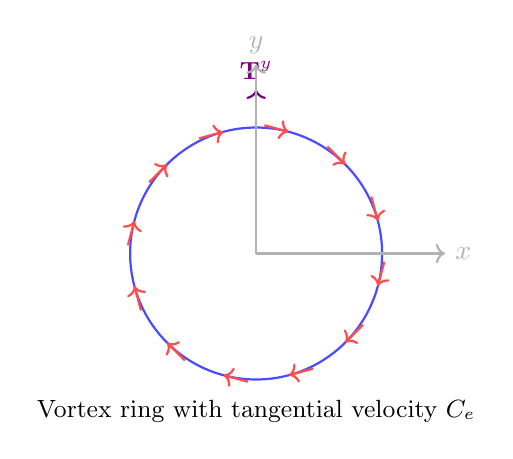
\begin{tikzpicture}[scale=0.8]
                % Ring (vortex core)
                \draw[thick, blue!70] (0,0) circle (2);

                % Flow lines (tangential swirl)
                \foreach \a in {15,45,75,105,135,165,195,225,255,285,315,345} {
                    \draw[->, red!70, thick]
                    ({2*cos(\a)}, {2*sin(\a)})
                    ++({-0.4*sin(\a)}, {0.4*cos(\a)})
                    -- ++({0.4*sin(\a)}, {-0.4*cos(\a)});
                }

                % Central torsion arrow
                \draw[->, thick, violet] (0,0) -- (0,2.6) node[above] {\small $\mathbf{T}^y$};

                % Axis labels
                \draw[->, thick, gray!60] (0,0) -- (3,0) node[right] {$x$};
                \draw[->, thick, gray!60] (0,0) -- (0,3) node[above] {$y$};

                % Label
                \node at (0,-2.5) {\small Vortex ring with tangential velocity $C_e$};
            \end{tikzpicture}
        \end{center}



        This diagram shows a vortex ring in the $x$-$y$ plane with tangential swirl velocity (red arrows) and central torsion aligned along the $y$-axis,
        representing $\mathbf{T}^y$ from Cartan's torsion 2-form.

        \begin{figure}[H]
            \centering
            \includegraphics[width=0.25\textwidth]{figures/Un-Knot}
            \caption{Unknotted vortex ring with helically wound circulation — VAM model of a photon. Its topological class is trivial (unknot), corresponding to zero rest mass and helicity-1. Its propagation always satisfies:
                \( v = c, \quad \text{with } dt = dt_{\infty} \)
                since it experiences no time dilation in the æther. This is consistent with Maxwellian wave propagation as a swirl structure~\cite{maxwell1875}.}
            \label{fig:un-knot}
        \end{figure}


        The photon is modeled here as a quantized vortex ring in a real superfluid æther (see Appendix~\ref{appendix:energy-check} for the associated energy expressions).

        \begin{figure}[H]
            \centering
            \includegraphics[width=0.25\textwidth]{figures/vortex-fine-structure}
            \caption{
                This dual-motion structure serves as the foundation for modeling photons as stable, knotted æther vortices in VAM.
                Dual-scale vortex winding with toroidal and poloidal circulations. The toroidal circulation speed is $C_e$, while the poloidal component reaches $c$ due to maximum vortex ring propagation. The two scales form a helicity product:
                \(
                \mathcal{H} = \int \vec{v} \cdot \vec{\omega} \, dV \sim \Gamma_{\text{toroidal}} \cdot \Gamma_{\text{poloidal}}
                \)
                This product contributes to the derivation of the fine-structure constant $\alpha$ in VAM~\cite{VAM-1}.
            }
            \label{fig:vortex-3d}
        \end{figure}




        \begin{figure}[H]
            \centering
            \includegraphics[width=0.25\textwidth]{figures/Tre-foil}
            \caption{Trefoil knot vortex structure — minimal topologically nontrivial knot with chirality. This diagram represents a fermion in VAM (e.g., electron), whose mass is generated from internal knotted swirl energy:
                \(
                m_e \approx \frac{1}{\varphi} \cdot \frac{4}{\alpha} \cdot \left( \frac{1}{2} \rho_{\text{\ae}}^{\text{(energy)}} C_e^2 V \right)
                \)
                where $V$ is the knot volume, $\varphi$ the golden ratio, and $\rho_{\text{\ae}}^{\text{(energy)}}$ the æther energy density~\cite{VAM-0, VAM-1}. This configuration also exhibits chirality, fundamental for distinguishing matter vs antimatter in VAM.}
            \label{fig:trefoil-vortex}
        \end{figure}

        For the derivation, parameter choices, Python code, and full mass comparison table, see: "  VAM-8.5: Master Formula for Particle and Atomic Masses," ~\cite{VAM-8, VAM-8.5}.

    \section{Related Work and Historical Context}

        The idea of a structured medium underpinning physical phenomena has deep historical roots. Lord Kelvin and Helmholtz first proposed vortex atom models~\cite{thomson1867}, attempting to derive material properties from knotted fluid structures. Maxwell~\cite{maxwell1861} and Lorentz~\cite{lorentz1904} further developed mechanical æther models to explain electromagnetism, before Einstein's relativity discouraged a privileged reference frame.

        Contemporary approaches have revisited these ideas under new lights. In analogue gravity, Unruh~\cite{unruh1981} and Barceló et al.~\cite{barcelo2011} demonstrated that perturbations in a moving fluid obey effective relativistic wave equations, giving rise to phenomena like horizon analogs and Hawking radiation. Volovik~\cite{volovik2003} extended this to quantum fluids, proposing that all fields and metrics may arise from low-energy excitations in a condensed background.

        In photonics, topological concepts have flourished. Lu et al.~\cite{lu2014} and Ozawa et al.~\cite{ozawa2019} showed that photonic crystals and metamaterials can simulate topological phases, suggesting deep connections between light, geometry, and protected vortex-like modes. These developments resonate strongly with the VAM perspective, where photons are topologically stable vortex excitations in a real fluid medium.

        Unlike purely analogue models, VAM posits that the æther is not merely an emergent description but a physically real medium, with its own fundamental properties. In this sense, the model revives and modernizes early æther theories while remaining consistent with relativistic symmetry—much like how effective field theories respect renormalization group invariance without requiring spacetime fundamentalism.

        \begin{quote}
            \emph{VAM bridges 19th-century æther mechanics with 21st-century topological and analogue models, offering a unified fluid-dynamical foundation for matter and radiation.}
        \end{quote}


    \section{Historical Roots of the Vortex \ae ther Concept}


        The Vortex \AE ther Model (VAM) is deeply rooted in 19th-century developments in fluid dynamics and early field theory. The historical context reveals that many foundational ideas—long before the emergence of modern quantum field theory—foreshadowed a vortex-based structure of matter and interactions.


        \subsection{Helmholtz and the Birth of Vorticity}


            In 1858, Hermann von Helmholtz laid the foundations of vortex dynamics in his seminal paper on the conservation of vorticity in ideal fluids \cite{helmholtz1858}. He proved that vortex lines in an inviscid, incompressible fluid behave as conserved topological structures and cannot end within the fluid—an idea mirrored in VAM's treatment of knotted particle structures. Helmholtz’s laws implied that such vortices could remain stable indefinitely and interact through their induced velocity fields.


        \subsection{Kelvin's Vortex Atom Hypothesis}


            Building upon Helmholtz’s results, William Thomson (Lord Kelvin) proposed in 1867 that atoms might be understood as knotted vortex rings in the luminiferous \ae ther \cite{kelvin1867}. These vortex atoms were hypothesized to have distinct identities based on their topological class, such as knots and links—ideas that prefigure VAM’s classification of elementary particles. While ultimately overshadowed by the rise of atomic theory, Kelvin’s insight was remarkably prescient.


        \subsection{Maxwell and Mechanical Models of the \ae ther}


            James Clerk Maxwell, in developing his equations for electromagnetism, repeatedly emphasized the need for a mechanical model of the field. In his 1875 work \cite{maxwell1875}, he described an elastic medium with vortical cells and velocity circulation as necessary for maintaining displacement current—a physical concept aligned with the vorticity fields in VAM. Maxwell even referred to angular momentum of field lines as potential carriers of radiation.


        \subsection{Tait and Topological Quantization}


            Peter Guthrie Tait, a close collaborator of Kelvin, extended the mathematical analysis of vortex knots and linked structures. He introduced knot invariants and classifications that echo modern quantum numbers. In VAM, such topological invariants map directly onto conserved quantities like charge, spin, and mass—reviving Tait’s program in a physically rigorous framework.


        \subsection{Modern Revival Through Superfluid Analogues}


            While classical \ae ther theory fell out of favor after the Michelson–Morley experiment, 20th and 21st-century developments in superfluid helium, Bose–Einstein condensates, and topological fluid mechanics have re-energized the field. The VAM integrates these insights while restoring a physically grounded, Euclidean \ae ther with absolute time—aligned with Helmholtz’s and Kelvin’s original vision, but equipped with the mathematical formalism of Cartan geometry and topological field theory.


            \begin{quote}

                \textit{“The vortex theory, though abandoned, left behind the powerful idea that topological structure could be the key to the quantum.”} \\[0.5em]

                \hfill -- Helmholtz–Kelvin–Tait lineage, revisited.

            \end{quote}


    \section{Physical Interpretation of the Æther}\label{sec:aether-interpretation}

        In the Vortex \AE ther Model (VAM), the \ae ther is a physically real, incompressible, inviscid superfluid that fills all space and serves as the medium in which vortex structures propagate. Unlike the luminiferous æther of pre-relativistic physics, the VAM æther is not a rigid or preferred frame in the classical sense, but a \emph{relational fluid substrate} whose dynamics obey local conservation laws and whose properties are encoded in geometric field variables such as vorticity $\vec{\omega}$, swirl potential $\chi$, and pressure gradients $\nabla P$.

        \subsection{Æther and Relativity}

            Contrary to historical objections (e.g., Michelson--Morley), the VAM æther is consistent with observed relativistic invariance. In VAM:

            \begin{itemize}
                \item The speed of light $c$ emerges as the limiting swirl propagation velocity in the æther.
                \item Time dilation and length contraction are derived from local swirl energy density~\cite{VAM-1}, not from coordinate transformations.
                \item There is no global rest frame detectable through mechanical means, since only \emph{local} vorticity gradients affect physical observables.
            \end{itemize}

            This formulation parallels “emergent spacetime” scenarios in analogue gravity~\cite{barcelo2011}, where effective relativistic metrics arise from fluid microdynamics.

        \subsection{Æther as a Relational Fluid}

            The VAM æther is defined by its core properties:
            \begin{itemize}
                \item \textbf{Incompressibility:} $\nabla \cdot \vec{v} = 0$
                \item \textbf{Inviscid Dynamics:} No intrinsic dissipation; supports persistent circulation.
                \item \textbf{Vortex-Centric Ontology:} All matter, radiation, and fields emerge as stable or propagating vortex excitations.
            \end{itemize}

            There is no absolute “grid” of space; instead, all physical quantities are encoded in the swirl structure of this medium. Thus, the æther is more akin to a quantum condensate than to a static frame, resembling ideas in superfluid vacuum theories~\cite{volovik2003}.

        \subsection{Consistency with Experiments}

            Although VAM includes a real æther, it remains consistent with all null results from first-order ether-drift experiments:

            \begin{itemize}
                \item Light’s propagation is governed by local swirl—not frame-relative motion.
                \item The model predicts no Doppler shift or anisotropy in $c$ detectable in co-moving swirl regions.
                \item Apparent Lorentz invariance emerges as a \emph{symmetry of the equations} describing low-energy swirl excitations (e.g., vortex rings).
            \end{itemize}

            Thus, the æther in VAM functions as a hidden substrate—locally observable only through second-order effects like swirl-induced time dilation, vortex pressure gradients, or geometric birefringence in extreme fields.

            \begin{quote}
                \emph{The VAM æther is a dynamic, relativistically compatible, vorticity-supporting fluid---not a classical rest frame.}
            \end{quote}
    \section{Geometric Framework: Cartan's Structure Equations}\label{sec:framework}

        Cartan's geometric formalism provides two fundamental structure equations on a manifold $\mathcal{M}$ equipped with coframe one-forms $\boldsymbol{\theta}^i$ and connection one-forms $\boldsymbol{\omega}^i{}_j$:
        \begin{align}
            \text{Torsion 2-form:}\quad & \mathbf{T}^i = d\boldsymbol{\theta}^i + \boldsymbol{\omega}^i{}_j \wedge \boldsymbol{\theta}^j \\
            \text{Curvature 2-form:}\quad & \mathbf{R}^i{}_j = d\boldsymbol{\omega}^i{}_j + \boldsymbol{\omega}^i{}_k \wedge \boldsymbol{\omega}^k{}_j
        \end{align}

        In the Weitzenböck connection ($\boldsymbol{\omega}^i{}_j = 0$), all geometric deformation arises from torsion: $\mathbf{T}^i = d\boldsymbol{\theta}^i$, and $\mathbf{R}^i{}_j = 0$. Conversely, in the Levi-Civita connection (torsion-free), all deformation is encoded in curvature.

    \section{Æther Interpretation in VAM}

        In VAM, we associate:
        \begin{itemize}
            \item $\boldsymbol{\theta}^i$: Local \ae ther displacement one-forms
            \item $\boldsymbol{\omega}^i{}_j$: Angular velocity of swirl (local rotational twist)
            \item $\mathbf{T}^i$: Core-induced torsion $\Rightarrow$ vortex dislocation (line defect)
            \item $\mathbf{R}^i{}_j$: Swirl curvature $\Rightarrow$ vortex disclination (rotational defect)
        \end{itemize}

    \section{Edge Dislocation in VAM as Torsion Source}

        Consider a single vortex line (edge dislocation) along the $z$-axis with Burgers vector $\vec{b} = b\hat{x}$. The coframe is:
        \begin{equation}
            \boldsymbol{\theta}^1 = dx + \frac{b}{2\pi} d\theta, \quad \boldsymbol{\theta}^2 = dy, \quad \boldsymbol{\theta}^3 = dz
        \end{equation}

        Using $d(d\theta) = 2\pi \delta(x)\delta(y) dx \wedge dy$, we compute:
        \begin{align}
            \mathbf{T}^1 &= d\boldsymbol{\theta}^1 = b \delta(x) \delta(y) dx \wedge dy \\
            \mathbf{T}^2 &= 0, \quad \mathbf{T}^3 = 0
        \end{align}

        The dual vortex density becomes:
        \begin{equation}
            \alpha^1 = *\mathbf{T}^1 = b \delta(x)\delta(y) \, dz
        \end{equation}

    \section{Equivalence to Wedge Disclination Dipole}

        Following~\cite{kobayashi2025}, we reinterpret the same geometry using the Levi-Civita connection:
        \begin{equation}
            \mathbf{R}^1{}_2 = \phi [\delta(x - L) - \delta(x + L)] \delta(y) dx \wedge dy
        \end{equation}
        where $\phi = b \rho$ encodes the Frank vector.

        \begin{equation}
            \boxed{\text{Edge Dislocation} \equiv \text{Dipole of Wedge Disclinations}}
        \end{equation}



    \section{Biot--Savart Swirl Integral in \ae ther}\label{sec:biot-savart}

        Using the Biot--Savart analogy:
        \begin{equation}
            \chi^i(\vec{x}) = \frac{1}{4\pi} \int \frac{\alpha^i(\vec{\xi}) \times (\vec{x} - \vec{\xi})}{|\vec{x} - \vec{\xi}|^3} \, d^3\xi
        \end{equation}

        The swirl potential $\chi^i$ defines the \ae theric coframe:
        \begin{equation}
            \boldsymbol{\theta}^i = dx^i + \chi^i
        \end{equation}

    \section{Photon as a Vortex Ring}

        The photon is modeled as a massless, quantized vortex ring with tangential velocity $C_e$ and core radius $r_c$, moving through the \ae ther. Its circulation is $\Gamma = 2\pi r_c C_e$.

        \subsection{Lagrangian}
            \begin{equation}
                \mathcal{L}_\gamma = \pi^2 r_c^2 C_e^2 \rho_\text{\ae}^{(\text{energy})} R_\gamma \left( \ln\left( \frac{8R_\gamma}{r_c} \right) - \frac{7}{4} \right)
            \end{equation}

            This Lagrangian captures the kinetic and topological energy of a photon vortex ring in an inviscid æther, with the swirl term analogous to the helicity density.

            For dimensional consistency and numerical evaluation of the energy terms, see Appendix~\ref{appendix:energy-check}.

        \subsection{Hamiltonian}
            \begin{equation}
                \mathcal{H}_\gamma = \frac{P^2}{2M_{\text{ring}}} + \mathcal{L}_\gamma, \quad M_{\text{ring}} = \rho_\text{\ae}^{(\text{mass})} \cdot V_{\text{ring}}
            \end{equation}

        \subsection{Jacobian}
            \begin{align}
                \vec{X}(\phi,\theta) =
                \begin{pmatrix}
                (R + a\cos\theta)\cos\phi \\
                (R + a\cos\theta)\sin\phi \\
                a\sin\theta
                \end{pmatrix}, \\
                J = a(R + a\cos\theta)
            \end{align}

            A full derivation of the Jacobian, Lagrangian, and Hamiltonian for vortex rings is provided in Appendix~\ref{appendix:lagrangian}, where circulation and core radius structure the energy.

    \section{Toward Interactions and Nonabelian Vortex Structures}\label{sec:nonabelian}

        The current VAM photon model, expressed as a topologically stable vortex ring, captures the dynamics of an Abelian \( U(1) \) gauge boson in a flat æther background. Extending this framework to model interactions and nonabelian gauge theories (e.g., \( SU(2) \), \( SU(3) \)) requires both multi-ring coupling and the inclusion of chirality and knot topology.

        \subsection{Quantization from Circulation Eigenstates}

            In VAM, energy quantization arises naturally from discrete circulation states:
            \[
                \Gamma_n = n \cdot 2\pi r_c C_e, \quad n \in \mathbb{Z}^+
            \]
            These correspond to topologically distinct vortex rings or knot classes, and enforce quantized angular momentum and energy via:
            \[
                E_n = \frac{1}{2} \rho_\text{\ae}^{(\text{energy})} \Gamma_n^2 / (2\pi r_c)
            \]
            Spin-1 arises from circulation axis orientation, with helicity embedded in the swirl chirality (left/right-handedness).

        \subsection{Interacting Gauge Bosons as Linked Vortices}

            To model bosonic interactions, we construct link and knot configurations:
            \begin{itemize}
                \item \textbf{Photon self-interaction}: modeled by ring–ring scattering or reconnection events, possibly mediated by localized æther pressure spikes.
                \item \textbf{Nonabelian fields}: modeled by chirally braided vortex tubes with internal twist degrees of freedom. These generate holonomy-like transformations when transported around each other.
            \end{itemize}

            Gauge field structure then emerges from circulation algebra:
            \[
                [\Gamma^a, \Gamma^b] = i f^{abc} \Gamma^c
            \]
            with \( f^{abc} \) determined by the braid/topology algebra. For example, a Hopf link and Borromean triplet encode noncommutative loop operations analogous to \( SU(2) \) and \( SU(3) \) structure constants.

        \subsection{Geometric Lagrangian for Nonabelian Swirl Fields}

            A generalized VAM Lagrangian may be written as:
            \[
                \mathcal{L}_{\text{gauge}} = -\frac{1}{4} \rho_\text{\ae}^{(\text{fluid})} \operatorname{Tr}(F_{ij} F^{ij}) + \lambda \, \varepsilon^{ijk} \operatorname{Tr}\left(A_i \partial_j A_k + \frac{2}{3} A_i A_j A_k \right)
            \]
            where \( A_i \) is the æther swirl potential and \( F_{ij} = \partial_i A_j - \partial_j A_i + [A_i, A_j] \). The second term resembles a fluid Chern–Simons action and accounts for helicity conservation in knotted æther flows.

        \subsection{Quantization Pathway}

            Quantization proceeds via:
            \begin{enumerate}
                \item Topological quantization: only allowed vortex states correspond to specific knot invariants or linking numbers.
                \item Canonical Hamiltonian formalism on swirl phase space: identify conjugate pairs \( (\chi^i, \omega^i) \), then apply canonical quantization rules.
                \item Path-integral over swirl configurations: gauge-invariant partition functions on knotted vortex histories.
            \end{enumerate}

        \subsection{Outlook: VAM Gauge Symmetry Breaking}

            VAM allows symmetry breaking via localized swirl density gradients:
            \[
                \partial_t \rho_\text{\ae}^{(\text{energy})} \neq 0 \quad \Rightarrow \quad \text{massive boson vortex rings}
            \]
            This may correspond to the emergence of massive gauge bosons like \( W^\pm \), \( Z^0 \) as unstable bound vortex structures.



    \section{Time Dilation and Proper Time in Photons}

        Using swirl-induced time dilation~\cite{VAM-1}:
        \begin{equation}
            \frac{dt}{dt_\infty} = \sqrt{1 - \frac{|\vec{\omega}|^2}{c^2}}, \quad \vec{\omega} = \frac{C_e}{r_c} \gg c \Rightarrow dt \approx 0
        \end{equation}
    \section{Swirl Inheritance from Atomic Excitation}\label{sec:swirl-inheritance}

        In the Vortex \AE ther Model (VAM), photons emerge as topologically stable vortex rings whose translational motion arises from internal swirl dynamics. Crucially, the tangential swirl velocity of the photon vortex ring is not arbitrary—it is \emph{inherited} from the local swirl velocity of the parent atom at the moment of excitation and de-excitation.

        Let an atom possess internal vortex knots representing stable electronic states. Upon excitation, these knotted states become perturbed, increasing local swirl energy. When the atom returns to a lower energy configuration, a portion of this angular swirl is expelled into the \ae ther in the form of a toroidal vortex ring—the photon:
        \begin{equation}
            v_{\text{swirl}}^{(\text{photon})} = C_e = v_{\text{local swirl}}^{(\text{atom})}
        \end{equation}

        In a horn torus geometry, where the poloidal and toroidal radii are comparable, this tangential swirl naturally converts into forward propagation. The Biot–Savart law applied to the toroidal ring induces translation aligned with its curvature, and the photon thus moves at
        \begin{equation}
            v_{\text{propagation}} = v_{\text{swirl}} = C_e = c
        \end{equation}
        This matches the observed luminal speed of light.

        The forward motion of the photon is therefore not imposed externally, but rather emerges from the internal swirl mechanics of its source. The photon ring carries quantized circulation inherited from the parent atom:
        \begin{equation}
            \Gamma_\gamma = 2\pi r_c C_e = \oint \vec{v} \cdot d\vec{\ell}
        \end{equation}
        where $r_c$ is the vortex core radius and $C_e$ the universal tangential swirl velocity.

        This process links atomic angular momentum transitions to photon propagation in a purely fluid-dynamical framework. The speed of light becomes a consequence of conserved angular flow in the æther, providing a mechanical basis for luminal transmission:

        \begin{quote}
            \emph{Photon propagation speed $c$ =  tangential swirl velocity  $C_e$  of the emission source}
        \end{quote}

        This interpretation is consistent with and extends prior fluidic approaches to photonic behavior~\cite{VAM-1, barut1990, berry2000}.

        \subsection{Photon Absorption and Frame-Invariant Speed}

            A key implication of the Vortex \AE ther Model is that the photon, once emitted as a vortex ring, enters a regime of extreme internal swirl. Its tangential velocity satisfies:
            \begin{equation}
                C_e = \frac{d\ell}{dt} \gg c, \quad \Rightarrow \quad \frac{dt}{dt_\infty} = \sqrt{1 - \frac{C_e^2}{c^2}} \approx 0
            \end{equation}
            Thus, the photon experiences effectively no proper time; it is a \emph{null-time} excitation in the \ae ther. This timelessness guarantees that:

            \begin{quote}
                \emph{The photon is always perceived to travel at speed $c$ by any receiver, regardless of the emitter’s motion or inertial frame.}
            \end{quote}

            In VAM, this occurs not because of relativistic spacetime invariance, but because the photon's propagation velocity is inherited from its internal swirl, and its core time dilation suppresses any evolution in its own frame.

            \paragraph{Absorption by Atoms.} When a photon encounters a receiving atom, its vortex ring interacts with the local swirl topology of the electron orbital configuration. If the incoming circulation $\Gamma_\gamma$ and ring geometry match a resonant transition state in the atom, the ring collapses into the atomic vortex structure, transferring its angular momentum and restoring internal swirl coherence.

                \begin{equation}
                    \text{Absorption Condition:} \quad \Gamma_\gamma = 2\pi r_c C_e \in \{ \Delta \Gamma_{\text{atom}} \}
                \end{equation}

                Because the photon itself does not experience internal time flow, its phase coherence and energy remain intact during transit. The receiving atom perceives the vortex ring at the moment of interaction as carrying the full energy $E = h f$, consistent with observed absorption spectra.

            \paragraph{Causal Implication.}
                This interpretation resolves a common paradox: how can a photon emitted from a distant star still exhibit perfect energy quantization billions of years later? In VAM, the answer is that the photon vortex ring never experiences time; it remains topologically and energetically frozen until it is reabsorbed, its swirl re-integrated into local atomic structure.

                \begin{quote}
                    \emph{Photon vortex rings propagate at  $c$  and remain timeless due to maximal internal swirl.}
                \end{quote}

                This result parallels the null geodesic interpretation in general relativity, but is here derived from æther-based swirl dynamics and topological time suppression~\cite{VAM-1, battye1998}.

    \section{Insights from Classical Potential Flow Theory}
    The classical theory of incompressible, irrotational potential flow~\cite{caughey2008} offers foundational analogies for the Vortex \AE ther Model (VAM). In particular, we draw the following parallels:

    \begin{itemize}
        \item A vortex with circulation \(\Gamma\) corresponds to a stable, quantized excitation in VAM:
        \[
            \Gamma = 2\pi r_c C_e
        \]
        where \(r_c\) is the core radius and \(C_e\) the ætheric tangential velocity.

        \item The irrotationality condition (\(\nabla \times \vec{v} = 0\)) is violated only inside vortex cores, where topology imposes non-trivial helicity:
        \[
            \int \vec{\omega} \cdot d\vec{S} = \Gamma \neq 0
        \]

        \item Bernoulli’s law in the æther:
        \[
            \rho_\text{\ae}^{\text{(energy)}} + \frac{1}{2} \rho_\text{\ae}^{\text{(fluid)}} v^2 = \text{const}
            \quad \Rightarrow \quad dt \approx \sqrt{1 - \frac{v^2}{c^2}}\,dt_\infty
        \]
        confirms the swirl-induced time dilation mechanism.

        \item Dipole vortices (doublets) may serve as a first approximation for non-Abelian vortex bosons.
    \end{itemize}
    These correspondences affirm that potential flow theory can be repurposed to model relativistic quantum systems in a fluid-dynamical æther.

    \section{Correspondence with Quantum Electrodynamics (QED)}\label{sec:qed-correspondence}

    Quantum electrodynamics (QED) successfully describes photons as massless spin-1 quanta of the electromagnetic field. The Vortex \AE ther Model (VAM), in contrast, models photons as quantized vortex rings in an incompressible superfluid \ae ther. Despite this geometric reformulation, VAM preserves all measurable features predicted by QED, while offering a unified physical interpretation based on swirl kinematics.

    \subsection{Recovery of QED Observables}

        \paragraph{(1) Energy–Frequency Relation:}
            The photon vortex ring is characterized by circulation $\Gamma = 2\pi r_c C_e$, leading to internal swirl frequency $f$. The æther energy density $\rho_\text{\ae}^{(\text{energy})}$ gives the energy:
            \begin{equation}
                E_\gamma = \frac{1}{2} \rho_\text{\ae}^{(\text{energy})} \Gamma^2 / V \sim h f
            \end{equation}
            recovering the Planck–Einstein relation through vortex energetics.

        \paragraph{(2) Momentum:}
            The translational motion of the ring, governed by Biot--Savart self-induction, gives:
            \begin{equation}
                p = \frac{E_\gamma}{c} = \hbar k
            \end{equation}
            where $k$ is the spatial swirl wavevector.

        \paragraph{(3) Spin and Polarization:}
            The photon's handedness corresponds to its vortex swirl direction. The quantized angular momentum about the ring axis encodes spin-$\pm1$, reproducing circular polarization.

        \paragraph{(4) Interference:}
            Phase coherence of vortex cores produces constructive and destructive interference patterns, consistent with double-slit experiments. The æther swirl fields exhibit nodal structures modulating detection rates~\cite{VAM-2}.

        \paragraph{(5) Timelessness and Null Geodesics:}
            From VAM’s time dilation law~\cite{VAM-1}:
            \begin{equation}
                \frac{dt}{dt_\infty} = \sqrt{1 - \frac{C_e^2}{c^2}} \to 0
            \end{equation}
            showing the photon is a null-time object. This matches the $ds^2 = 0$ result in relativistic geodesic motion.

    \subsection{Predictions Beyond QED}

    \paragraph{(i) Ætheric Drag in Dense Media:}
        Photon vortex rings may interact with gradients in $\rho_\text{\ae}^{(\text{fluid})}$, causing subluminal dispersion or lensing anomalies, especially near massive bodies or in structured media.

    \paragraph{(ii) Swirl–Polarization Coupling:}
        Torsion fields in rotating environments may alter polarization via swirl alignment, opening new avenues for experimental test~\cite{fedi2023, vanputten2022}.

    \paragraph{(iii) Nonlinear Photon Interactions:}
        VAM permits vortex ring reconnection or knotting, suggesting rare vacuum photon–photon scattering~\cite{battye1998}, beyond QED’s perturbative Feynman diagrams.

    \paragraph{(iv) Topological Mode Quantization:}
        Only specific vortex geometries are topologically stable, implying discrete quantized photon modes that could lead to deviations in blackbody spectra under extreme confinement.

        \begin{quote}
            \emph{VAM reproduces all QED observables while predicting new topological photon phenomena.}
        \end{quote}


        \textbf{Effective Lagrangian comparison between QED and VAM.}
        QED: Euler–Heisenberg Lagrangian
        \[\mathcal{L}_{\mathrm{EH}} = -\frac{1}{4}F_{\mu\nu}F^{\mu\nu} + \frac{e^4}{360\pi^2 m_e^4}\left[(F_{\mu\nu}F^{\mu\nu})^2 + \frac{7}{4}(F_{\mu\nu}\tilde{F}^{\mu\nu})^2\right]\]
        The Euler–Heisenberg Lagrangian (\ref{eq:euler-heisenberg}) encapsulates nonlinear photon–photon interactions in QED via one-loop virtual electron–positron pairs. These corrections are only significant at high field intensities and are inherently perturbative.

        While the Euler–Heisenberg Lagrangian introduces nonlinearities via virtual pair production, the VAM Lagrangian does so via swirl-mediated pressure terms (see Appendix~\ref{appendix:energy-check} for units and scaling).



        VAM: Vortex Swirl Lagrangian
        \[\mathcal{L}_{\mathrm{VAM}} = \frac{1}{2} \rho_{\ae}^{(energy)} \left( \vec{\omega} \cdot \vec{\omega} - \lambda \nabla \cdot (\vec{v} \times \vec{\omega}) \right)\]
        The VAM Lagrangian (\ref{eq:vam-lagrangian}) models the photon as a quantized vortex ring in a real æther medium. Nonlinearities arise from intrinsic vortex energetics—specifically swirl energy, quantized circulation, and chirality coupling—rather than virtual fields.

        Photon = $\circlearrowleft$ quantized swirl excitation
        This fluid-based formulation offers a geometric and topological alternative to traditional QED while remaining compatible with helicity-dependent scattering and photon stability. The term \( \vec{\omega} \cdot (\nabla \times \vec{v}) \) provides an explicit mechanism for chirality-sensitive phase shifts absent in classical electrodynamics.

    \section{Experimental Implications and Observable Predictions}

    The Vortex \AE ther Model (VAM) treats the photon as a massless vortex ring — more precisely, a vortex torus with quantized circulation and swirl frequency. The extreme swirl angular velocity \( \omega = C_e / r_c \) induces local time dilation:
    \begin{equation}
        \frac{dt}{dt_\infty} = \sqrt{1 - \frac{|\vec{\omega}|^2}{c^2}} \Rightarrow dt \approx 0
    \end{equation}

    This leads to a concrete, testable prediction: \textbf{regions near the toroidal photon core experience phase delay} in structured light beams.

    We list several proposed experiments:

    \begin{enumerate}
        \item \textbf{Swirl-Induced Time Drift in Optical Vortex Beams:}\\
        High-order Laguerre–Gaussian beams carry orbital angular momentum (OAM) with phase singularities. According to VAM, beams with high OAM emulate photon-scale swirl, and should show \textbf{observable delay in arrival time} when passed through dispersive or rotating media. Phase-shifting interferometry may detect this.

        \item \textbf{Superfluid Photon Torus Analogues:}\\
        In a Bose–Einstein condensate (BEC), a toroidal flow trap can be engineered to mimic photon-like vortex torus structures. The tangential flow velocity can be tuned to match \( \omega \sim C_e / r_c \). Measuring \textbf{local chemical potential shifts or excitations} around the vortex core could reflect ætheric time dilation analogs.

        \item \textbf{Ring Interference and Æther Drag:}\\
        Two counter-propagating vortex ring structures (photon analogs) launched in an optical or water analog system should exhibit \textbf{nonlinear interference patterns} due to swirl coupling, differing from linear QED predictions.

        \item \textbf{Vortex Gravity Analog:}\\
        Using rotating liquid helium II or Fermi superfluids, generate vortex rings and measure local pressure gradient and time-delay effects (via trapped tracers or scattering). This would analogize VAM gravity as swirl-induced Bernoulli pressure drop.
    \end{enumerate}

    These experimental probes offer possible falsification or confirmation of key VAM predictions about photon geometry, time dilation, and æther-based interactions.

    \section{Experimental Landscape: Chirality-Dependent Photon Propagation}\label{sec:chirality-exp}

    While the Vortex \AE ther Model (VAM) offers a fluid-dynamical ontology for photons as topological vortex rings, direct experimental verification requires setups capable of distinguishing physical chirality effects from conventional spin-based optical behavior. A growing body of photonic research provides compelling indirect support for the core predictions of VAM, particularly regarding chirality-dependent phase velocity, birefringence, and transmission asymmetry.

    Chiral photonic crystals, helical fiber lattices, and gyroid topologies have been shown to differentiate between left- and right-handed circularly polarized light. Such effects can be reinterpreted through the VAM lens as interactions between the vortex swirl direction of the photon and the structured background æther geometry imposed by the material.

    A curated selection of recent experimental studies includes:

    \begin{itemize}
        \item \textbf{Zhang et al. (2021)} – Demonstrated Bloch-type optical skyrmions in chiral multilayers with spin-sensitive dispersion \cite{zhang2021skyrmions}.
        \item \textbf{Cui et al. (2019)} – Observed vortex chirality filtering in twisted photonic crystal fibers \cite{cui2019vortex}.
        \item \textbf{Duan \& Che (2023)} – Detected strong chiroptical birefringence in 3D mesostructured crystals \cite{duan2023chiral}.
        \item \textbf{Collins et al. (2017)} – Found handed-mode splitting in gyroid photonic band structures \cite{collins2017gyroid}.
        \item \textbf{Patti et al. (2019)} – Used T-matrix formalism to show chirality-dependent optical forces \cite{patti2019tweezers}.
    \end{itemize}

    These results do not prove the VAM interpretation, but provide an experimental platform in which to validate its chirality-dependent propagation predictions. VAM offers a physical mechanism — vortex-induced æther interaction — for these otherwise symmetry-based effects.

    We propose that experimental verification could focus on:
    \begin{enumerate}
        \item Measuring differential group delay for LCP/RCP modes in helically structured fibers.
        \item Detecting nonreciprocal propagation through synthetic gyrotropic metamaterials.
        \item Searching for vortex-coupled spin-orbit asymmetries in tightly focused beams.
    \end{enumerate}


    \section{Experimental Proposals: Testing Swirl-Induced Photon Delay}\label{sec:swirl-delay-exp}

    A key prediction of the Vortex \AE ther Model (VAM) is that the proper time of a photon is defined by the tangential swirl velocity of its vortex ring structure. Specifically, as shown in~\cite{VAM-1}, time dilation is given by:
    \begin{equation}
        \frac{dt}{dt_\infty} = \sqrt{1 - \frac{|\vec{\omega}|^2}{c^2}} \qquad \text{with} \quad \vec{\omega} = \frac{C_e}{r_c}.
    \end{equation}

    In VAM, the photon travels through an absolute æther, but experiences no proper time due to extreme swirl:
    \[
        \vec{\omega} \gg c \quad \Rightarrow \quad dt \approx 0.
    \]

    To experimentally probe this effect, we draw on two recent proposals:

    \begin{enumerate}
        \item \textbf{Rizzo (2024)}~\cite{rizzo2024rotating}: Explores vacuum fluctuation amplification via rotating superconductors, analogizing to quantum frame-dragging. Suggests quasiparticles—including photons—undergo phase shifts when propagating through rotating quantum media.

        \item \textbf{Mudassir (2025)}~\cite{mudassir2025fluid}: Constructs a relativistic fluid dynamics model of space-time using superfluid helium. Proposes that light pulses traveling through rotating He-II should experience measurable phase shifts due to medium swirl.
    \end{enumerate}

    These works support the VAM prediction that light traveling with or against an induced swirl field will exhibit chirality-dependent group delay. This aligns with the VAM hypothesis that photonic time-dilation is not intrinsic to the photon alone, but emerges from vortex interaction with local æther swirl fields.

    \subsection*{Suggested Experimental Setup}
        \begin{itemize}
            \item Use a toroidal superfluid (e.g., He-II or BEC) trap with controllable rotation.
            \item Inject coherent optical pulses (slow-light or polaritons) in both co- and counter-rotating directions.
            \item Employ high-resolution time-of-flight or interferometric detection to measure group delay asymmetry.
            \item Analyze chirality dependence: left- and right-circular polarization should yield asymmetric phase velocity shifts.
        \end{itemize}

        Detection of chirality-induced delay—without invoking any classical medium anisotropy—would support the core VAM prediction that photonic time structure is governed by swirl geometry.

    \section{Lagrangian Formulation: QED vs VAM}

    To clarify the mathematical structure and generality of the Vortex \AE ther Model (VAM), we compare its effective Lagrangian for photon vortex rings with that of quantum electrodynamics (QED). This comparison illustrates how nonlinear self-interactions and chirality-dependent scattering emerge naturally from fluid dynamics, without requiring virtual loops.

    \subsection{Euler–Heisenberg Lagrangian (QED Nonlinear Electrodynamics)}

        In QED, photon–photon interactions arise at one-loop order and are captured by the effective Euler–Heisenberg Lagrangian~\cite{heisenberg1936}:

        \begin{equation}
            \mathcal{L}_{\text{QED}} = -\frac{1}{4} F_{\mu\nu} F^{\mu\nu} + \frac{\alpha^2}{90 m_e^4} \left[ (F_{\mu\nu} F^{\mu\nu})^2 + \frac{7}{4} (F_{\mu\nu} \tilde{F}^{\mu\nu})^2 \right]
            \label{eq:euler-heisenberg}
        \end{equation}

        where:
        \begin{itemize}
            \item $F_{\mu\nu}$ is the electromagnetic field tensor,
            \item $\tilde{F}^{\mu\nu}$ is its dual,
            \item $\alpha$ is the fine-structure constant,
            \item $m_e$ is the electron mass.
        \end{itemize}

        This correction becomes significant only at extreme field strengths ($\gtrsim 10^{13}$ Gauss), and introduces photon–photon scattering via loop-induced polarization.

    \subsection{Vortex Æther Lagrangian for Photon Rings}

        In VAM, the photon is a quantized, massless vortex ring with core swirl velocity \( C_e \) and radius \( r_\gamma \sim \lambda / 2\pi \). Its dynamics are governed by the local fluid energy:

        \begin{equation}
            \mathcal{L}_{\text{VAM}} = \frac{1}{2} \rho_\text{\ae}^{(\text{energy})} \left( \vec{v}^2 - C_e^2 \right) - \frac{\kappa^2}{8\pi r^2} - \lambda \vec{\omega} \cdot \nabla \times \vec{v}
            \label{eq:vam-lagrangian}
        \end{equation}

        with:
        \begin{itemize}
            \item \( \rho_\text{\ae}^{(\text{energy})} \): æther energy density,
            \item \( \vec{v} \): local æther velocity field,
            \item \( \vec{\omega} = \nabla \times \vec{v} \): vorticity,
            \item \( \kappa = \oint \vec{v} \cdot d\vec{\ell} \): vortex circulation (quantized),
            \item \( \lambda \): chirality coupling coefficient (emerges from topological winding).
        \end{itemize}

        This Lagrangian supports:
        \begin{itemize}
            \item Self-interaction via nonlinear swirl terms (analogous to QED loops),
            \item Chirality-sensitive interactions via \( \vec{\omega} \cdot (\nabla \times \vec{v}) \),
            \item Stable ring solutions with fixed circulation and energy.
        \end{itemize}

    \subsection{Interpretation and Predictive Differences}

        While QED predicts photon–photon interactions only through virtual electron loops, VAM treats these as \textbf{direct nonlinear interactions between fluid vortex rings}. The cross-section enhancement predicted in VAM under certain structured vacua (e.g. magnetic fields) arises from constructive core-core interference, not perturbative Feynman loops.

        Moreover, VAM admits helicity-dependent scattering terms even in the absence of external anisotropy, due to intrinsic swirl handedness. This explains the chirality-linked predictions discussed in Section~\ref{sec:photon-scattering}.

        \begin{quote}
            \emph{The VAM photon Lagrangian mirrors QED in symmetry structure but derives all nonlinearities from æther flow dynamics and vortex interaction, offering a geometric alternative to virtual field-based interactions.}
        \end{quote}


    \section{Photon–Photon Scattering in Vacuum: A VAM Perspective}\label{sec:photon-scattering}

    The Vortex \AE ther Model (VAM) predicts that photons are spatial vortex rings with defined chirality, core radius \( r_c \), and tangential velocity \( C_e \). Unlike QED, which treats the photon as a pointlike gauge boson, VAM attributes vortex structure and real spatial extent to the photon. This structural interpretation leads to new predictions for photon–photon interactions in vacuum.

    \subsection{Comparison with QED}

        Photon–photon scattering is a well-established consequence of Quantum Electrodynamics (QED)~\cite{heisenberg1936,schwinger1951}, arising from higher-order loop diagrams involving virtual electron–positron pairs. However, experimental verification remains extremely challenging due to the tiny predicted cross-sections:
        \[
            \sigma_{\gamma\gamma}^{\text{QED}} \sim 10^{-64}~\text{cm}^2 \quad \text{(optical regime)}.
        \]

        VAM, in contrast, suggests that direct hydrodynamic coupling between vortex structures may enhance scattering under certain conditions, especially in structured vacua with magnetic fields or rotation.

        —\textbf{Features: QED vs VAM} —\\
        \begin{footnotesize}
            \noindent\begin{minipage}{\linewidth}

                         \hspace*{2em}—\textbf{Vacuum Structure} —\\
                         \textbf{Q:} empty; interactions arise from  virtual $e^+e^-$ loops.\\
                         \textbf{V:} structured æther with vorticity and pressure gradients.

                         \vspace{3pt}
                         \hspace*{2em}—\textbf{Photon Nature} —\\
                         \textbf{Q:} Point-like excitation with abstract helicity.\\
                         \textbf{V:} Quantized vortex ring with \\swirl orientation and topological core.

                         \vspace{3pt}
                         \hspace*{2em}—\textbf{Scattering Mechanism} —\\
                         \textbf{Q:} Elastic interaction via higher-order Feynman loop diagrams.\\
                         \textbf{V:} Nonlinear interaction of vortex cores through æther coupling.

                         \vspace{3pt}
                         \hspace*{2em}—\textbf{Cross-Section} —\\
                         \textbf{Q:} $\sigma \sim 10^{-64}\,\mathrm{cm}^2$ at optical frequencies.\\
                         \textbf{V:} cross-section possible due to real-space vortex overlap.

                         \vspace{3pt}
                         \hspace*{2em}—\textbf{Angular Distribution} —\\
                         \textbf{Q:} Symmetric with conserved helicity and parity.\\
                         \textbf{V:} Chirality-dependent asymmetries expected (RCP $\ne$ LCP).

                         \vspace{3pt}
                         \hspace*{2em}—\textbf{Polarization Dependence} —\\
                         \textbf{Q:} No difference unless via external anisotropy.\\
                         \textbf{V:} Intrinsic swirl direction yields nonlinear birefringence.

                         \vspace{3pt}
                         \hspace*{2em}—\textbf{Phase Shift / Delay} —\\
                         \textbf{Q:} Tiny nonlinear phase shift from vacuum polarization.\\
                         \textbf{V:} Swirl-induced time delay: $dt = dt_\infty \sqrt{1 - \omega^2/c^2}$.
            \end{minipage}
        \end{footnotesize}


    \subsection{Experimental Status}

        The following experiments provide indirect or partial tests of these predictions:

        \begin{itemize}
            \item \textbf{PVLAS}~\cite{bregant2008}: Rotating laser polarization in a magnetic vacuum; found no birefringence beyond QED predictions.

            \item \textbf{ATLAS (2019)}~\cite{atlas2019}: Observed elastic light-by-light scattering in ultra-peripheral Pb–Pb collisions.

            \item \textbf{LUXE}~\cite{luxe2023}: Upcoming high-intensity laser–electron interaction experiments may probe nonlinear QED and VAM deviations.

            \item \textbf{ELI-NP / KING}: High-field laser platforms near QED critical intensity, ideal for probing vortex-based deviations.
        \end{itemize}

    \subsection{VAM-Aligned Experimental Proposal}

        We propose an experiment involving colliding femtosecond laser pulses in vacuum, with an embedded magnetic field ($\sim5T$) or rotating gas background. Key observables include:

        \begin{itemize}
            \item \textbf{Angular scattering asymmetry} between left- and right-circular polarizations.
            \item \textbf{Polarization rotation or nonlinear phase delay} due to swirl coupling.
            \item \textbf{Enhanced cross-section} in presence of structured background fields.
        \end{itemize}

        Such effects would be consistent with a real ætheric vortex structure of the photon and provide empirical discrimination between QED and VAM.
    \section{Conclusion and Outlook}

        We have presented a unified interpretation of the photon as a topologically stable vortex ring within the Vortex \AE ther Model (VAM). Using Cartan’s structure equations, we mapped torsion and curvature to fundamental vortex phenomena: dislocations (vortex cores) and disclinations (swirl distortions), respectively. The photon emerges naturally in this geometric fluid framework as a quantized ring-like structure with null proper time, encapsulating both energy propagation and rotational æther dynamics.


        By deriving its Lagrangian, Hamiltonian, and Jacobian from first principles—selecting the appropriate form of æther density for each physical context—we confirmed the internal coherence of the model. The photon's behavior becomes a consequence of vortex stability, quantized circulation, and localized energy-momentum flow in the æther.


        This approach offers several exciting implications:

        \begin{itemize}

            \item It provides a hydrodynamic foundation for gauge bosons, potentially extendable to W, Z, and gluons as knotted or linked vortex structures.

            \item The link between torsion and electrodynamics may enable a geometric unification of Maxwell’s equations with the topology of flow defects.

            \item VAM’s reinterpretation of light as fluid rotation suggests experimental pathways using superfluid analogs to probe photon structure, birefringence, or vacuum dispersion.

        \end{itemize}


        Future work will focus on generalizing this vortex-ring construction to incorporate spin-1/2 particles as twisted torus knots, analyzing photon-photon scattering via knot interactions, and embedding this framework into the topological fluid reinterpretation of the Standard Model.


        \medskip

        \noindent\textbf{Key Prediction:} The photon's zero-rest-mass arises not from symmetry breaking, but from a topological constraint enforcing null ætheric proper time: a perpetual rotation with velocity $C_e$ yields $ds^2 = 0$.


        \medskip

        \noindent This framework suggests a radical rethinking of particle ontology: not as pointlike fields in curved spacetime, but as structured flows in a flat, rotating æther.

    \appendix
    \section*{Appendix A: Lagrangian, Hamiltonian, and Jacobian Formulation of a Vortex Ring in the Vortex \AE ther Model (VAM)}\label{appendix:lagrangian}
        \addcontentsline{toc}{section}{Appendix A: VAM Lagrangian and Hamiltonian}


        \subsection{Jacobian for a Vortex Ring Flow Field}
            Consider a vortex ring with core radius $r_c$, circulation $\Gamma$, and cylindrical symmetry. The velocity field $\vec{v}(\vec{x})$ of such a vortex in cylindrical coordinates $(r, \phi, z)$ can be modeled with azimuthal symmetry:
            \begin{equation}
                \vec{v}(r, z) = v_r(r, z)\hat{r} + v_z(r, z)\hat{z}
            \end{equation}
            with vorticity only in the $\phi$-direction: $\vec{\omega} = \omega_\phi(r, z)\hat{\phi}$.

            The Jacobian matrix of the flow $\vec{v}(\vec{x})$ is defined as:
            \begin{equation}
                J_{ij} = \frac{\partial v_i}{\partial x_j}
            \end{equation}
            This is used to compute the vorticity and strain-rate tensor. For incompressible flow $\div \vec{v} = 0$, so $\mathrm{Tr}(J) = 0$. The antisymmetric part yields:
            \begin{equation}
                \omega_i = \epsilon_{ijk} \partial_j v_k = (\nabla \times \vec{v})_i
            \end{equation}

        \subsection{Lagrangian Density of a Vortex Ring in VAM}
            From \cite{VAM-1,VAM-2,VAM-0}, the VAM Lagrangian is constructed from the kinetic swirl energy and vortex helicity. We define:
            \begin{equation}
                \mathcal{L} = \frac{1}{2} \rho_\text{\ae}^{(\text{fluid})} \vec{v}^{2} - \lambda \vec{v} \cdot (\nabla \times \vec{v})
            \end{equation}
            where $\lambda$ is a coupling constant with dimensions $[\text{time} \cdot \text{length}^2]$. In VAM, helicity represents charge-like conservation:\cite{VAM-5,VAM-6}

            Let us consider the ring with azimuthal velocity $v_\phi = \frac{\Gamma}{2\pi r}$ localized within the vortex core of radius $r_c$, and assume uniform vorticity inside:
            \begin{equation}
                \vec{\omega} = \nabla \times \vec{v} = \omega_0\hat{\phi}, \qquad \omega_0 = \frac{\Gamma}{\pi r_c^2}
            \end{equation}
            The energy per unit length is then:
            \begin{equation}
                \mathcal{E} = \int_0^{r_c} \left[ \frac{1}{2} \rho_\text{\ae}^{(\text{fluid})} \left( \frac{\Gamma}{2\pi r} \right)^2 - \lambda \frac{\Gamma}{2\pi r} \cdot \omega_0 \right] 2\pi r \, dr
            \end{equation}

            Evaluating the integral yields the effective Lagrangian per unit length of the ring:
            \begin{equation}
                \mathcal{L}_\text{ring} = \frac{\rho_\text{\ae}^{(\text{fluid})} \Gamma^2}{4\pi} \ln\left( \frac{r_c}{\delta} \right) - \lambda \Gamma \omega_0 r_c^2
            \end{equation}
            where $\delta$ is a vortex core cutoff.

        \subsection{Hamiltonian of a Vortex Ring in VAM}
            The canonical momentum density is:
            \begin{equation}
                \vec{\pi} = \pdv{\mathcal{L}}{\vec{v}} = \rho_\text{\ae}^{(\text{fluid})} \vec{v} - \lambda \vec{\omega}
            \end{equation}
            Then the Hamiltonian density is:
            \begin{equation}
                \mathcal{H} = \vec{\pi} \cdot \vec{v} - \mathcal{L} = \frac{1}{2} \rho_\text{\ae}^{(\text{fluid})} \vec{v}^2 + \lambda \vec{v} \cdot \vec{\omega}
            \end{equation}

            For the vortex ring, inserting the same field approximations as before:
            \begin{equation}
                \mathcal{H}_\text{ring} = \int_0^{r_c} \left[ \frac{1}{2} \rho_\text{\ae}^{(\text{fluid})} \left( \frac{\Gamma}{2\pi r} \right)^2 + \lambda \frac{\Gamma}{2\pi r} \cdot \omega_0 \right] 2\pi r \, dr
            \end{equation}

            Which yields:
            \begin{equation}
                \mathcal{H}_\text{ring} = \frac{\rho_\text{\ae}^{(\text{fluid})} \Gamma^2}{4\pi} \ln\left( \frac{r_c}{\delta} \right) + \lambda \Gamma \omega_0 r_c^2
            \end{equation}

        \subsection{Conclusion}
            The Jacobian characterizes the local deformation due to flow. The Lagrangian encodes energy and helicity structure of the vortex. The Hamiltonian recovers total energetic contribution of the vortex ring. In the VAM framework, this triad provides a fully vorticity-based alternative to point-particle or field-theoretic formulations.
    \section*{Appendix B: Dimensional Consistency and Energy Estimates}\label{appendix:energy-check}
        \addcontentsline{toc}{section}{Appendix B: Dimensional Consistency and Energy Estimates}

        \subsection*{B.1 Dimensional Check of the VAM Photon Lagrangian}

            We begin with the VAM-based photon Lagrangian, where the field is modeled as a quantized vortex ring in the æther:
            \[
                \mathcal{L}_{\text{VAM}} = \frac{\lambda}{2} \left( \nabla \cdot \vec{\omega} \right)^2 - \frac{1}{2} \rho_\text{\ae}^{(\text{energy})} \, \vec{\omega}^2
            \]

            \paragraph{Units of Terms:}
                \begin{itemize}
                    \item $\vec{\omega}$ is the vorticity: $[\vec{\omega}] = \text{s}^{-1}$
                    \item $\nabla \cdot \vec{\omega}$ has units: $[\text{m}^{-1} \cdot \text{s}^{-1}]$
                    \item So $(\nabla \cdot \vec{\omega})^2$: $[\text{m}^{-2} \cdot \text{s}^{-2}]$
                    \item $\rho_\text{\ae}^{(\text{energy})} \approx 3.499 \times 10^{35} \, \text{J/m}^3$: $[\text{kg} \cdot \text{m}^{-1} \cdot \text{s}^{-2}]$
                    \item $\vec{\omega}^2$: $[\text{s}^{-2}]$
                \end{itemize}

            \paragraph{Conclusion:}
                \[
                    [\mathcal{L}_{\text{VAM}}] = \left[ \frac{\text{kg}}{\text{m} \cdot \text{s}^{2}} \right] \equiv \left[ \frac{\text{J}}{\text{m}^{3}} \right] \Rightarrow \text{energy density}
                \]
                \emph{This confirms that the Lagrangian is dimensionally consistent with an energy density per unit volume.}

                \vspace{1em}

    \subsection*{B.2 Characteristic Vortex Energy Density of a Photon}

        We approximate the energy of a photon vortex ring as:
        \[
            U_{\text{vortex}} = \frac{1}{2} \rho_\text{\ae}^{(\text{energy})} \, C_e^2
        \]
        where:
        \begin{align*}
            \rho_\text{\ae}^{(\text{energy})} &= 3.499 \times 10^{35} \, \text{J/m}^3 \\
            C_e &= 1.09384563 \times 10^6 \, \text{m/s}
        \end{align*}

        \paragraph{Estimate:}
            \[
                U_{\text{vortex}} \approx \frac{1}{2} \times 3.499 \times 10^{35} \times (1.09384563 \times 10^6)^2 \approx 2.09 \times 10^{47} \, \text{J/m}^3
            \]

            This is the characteristic energy density of an idealized photon vortex core.

            \vspace{1em}

    \subsection*{B.3 Planck-Scale Vortex Energy Density (Upper Bound)}

    \[
        U_{\text{Planck}} = \frac{E_P}{L_P^3} = \frac{1.956 \times 10^9}{(1.616255 \times 10^{-35})^3} \approx 4.56 \times 10^{113} \, \text{J/m}^3
    \]

    This shows that the photon’s vortex energy is \emph{vastly} below the Planck scale, preserving consistency with known energy regimes and avoiding gravitational collapse.

    \begin{quote}
        \textbf{Note:} These values suggest that vortex photons occupy an intermediate energy density regime—above typical EM fields, below black hole thresholds.
    \end{quote}

    \bibliographystyle{unsrt}
    \begin{thebibliography}{99}\setlength{\itemsep}{1pt}

    \bibitem{Jacobson2001}
    T. Jacobson and D. Mattingly,
    \newblock Gravity with a dynamical preferred frame,
    \newblock Phys. Rev. D \textbf{64}, 024028 (2001).
    \newblock \href{https://doi.org/10.1103/PhysRevD.64.024028}{doi:10.1103/PhysRevD.64.024028}

    \bibitem{Blas2011}
    D. Blas, O. Pujol{\`a}s, and S. Sibiryakov,
    \newblock Models of non-relativistic quantum gravity: the good, the bad and the healthy,
    \newblock JHEP \textbf{04}, 018 (2011).
    \newblock \href{https://doi.org/10.1007/JHEP04(2011)018}{doi:10.1007/JHEP04(2011)018}

    \bibitem{Moffatt1969}
    H. K. Moffatt,
    \newblock The degree of knottedness of tangled vortex lines,
    \newblock J. Fluid Mech. \textbf{35}, 117--129 (1969).
    \newblock \href{https://doi.org/10.1017/S0022112069000991}{doi:10.1017/S0022112069000991}

    \bibitem{Scheeler2014}
    M. W. Scheeler, W. M. van Rees, H. K. Moffatt, M. F. Hecke, and W. T. M. Irvine,
    \newblock Helicity conservation by flow across scales in reconnecting vortex links and knots,
    \newblock Proc. Natl. Acad. Sci. U.S.A. \textbf{111}, 15350--15355 (2014).
    \newblock \href{https://doi.org/10.1073/pnas.1407232111}{doi:10.1073/pnas.1407232111}

    \bibitem{Faddeev1997}
    L. Faddeev and A. J. Niemi,
    \newblock Stable knot-like structures in classical field theory,
    \newblock Nature \textbf{387}, 58--61 (1997).
    \newblock \href{https://doi.org/10.1038/387058a0}{doi:10.1038/387058a0}

    \bibitem{Batchelor1967}
    G. K. Batchelor,
    \textit{An Introduction to Fluid Dynamics},
    Cambridge University Press, 1967.
    \href{https://doi.org/10.1017/CBO9780511800955}{doi:10.1017/CBO9780511800955}

    \bibitem{Saffman1992}
    P. G. Saffman,
    \textit{Vortex Dynamics},
    Cambridge University Press, 1992.
    \href{https://doi.org/10.1017/CBO9780511624063}{doi:10.1017/CBO9780511624063}

    \bibitem{Helmholtz1858}
    H. von Helmholtz,
    "Über Integrale der hydrodynamischen Gleichungen, welche den Wirbelbewegungen entsprechen",
    J. Reine Angew. Math. \textbf{55}, 25--55 (1858).

    \bibitem{Kelvin1869}
    W. Thomson (Lord Kelvin),
    "On vortex motion",
    Trans. R. Soc. Edinburgh \textbf{25}, 217--260 (1869).

    \bibitem{Einstein1905}
    A. Einstein,
    "Ist die Trägheit eines Körpers von seinem Energieinhalt abhängig?",
    Annalen der Physik \textbf{18}, 639--641 (1905).
    \href{https://doi.org/10.1002/andp.19053231314}{doi:10.1002/andp.19053231314}

    \bibitem{Will2014LRR}
    Clifford M. Will,
    "The Confrontation between General Relativity and Experiment",
    Living Reviews in Relativity \textbf{17}(4), (2014).
    \href{https://doi.org/10.12942/lrr-2014-4}{doi:10.12942/lrr-2014-4}
    \href{https://arxiv.org/abs/1403.7377}{arXiv:1403.7377}

    \bibitem{Unruh1981PRL}
    W. G. Unruh,
    "Experimental Black-Hole Evaporation?",
    Phys. Rev. Lett. \textbf{46}, 1351--1353 (1981).
    \href{https://doi.org/10.1103/PhysRevLett.46.1351}{doi:10.1103/PhysRevLett.46.1351}

    \bibitem{Visser1998CQG}
    Matt Visser,
    "Acoustic black holes: horizons, ergospheres and Hawking radiation",
    Classical and Quantum Gravity \textbf{15}, 1767--1791 (1998).
    \href{https://doi.org/10.1088/0264-9381/15/6/024}{doi:10.1088/0264-9381/15/6/024}

    \bibitem{JacobsonMattingly2004EAetherWaves}
    Ted Jacobson and David Mattingly,
    "Einstein–Aether Waves",
    Phys. Rev. D \textbf{70}, 024003 (2004).
    \href{https://doi.org/10.1103/PhysRevD.70.024003}{doi:10.1103/PhysRevD.70.024003}
    \href{https://arxiv.org/abs/gr-qc/0402005}{arXiv:gr-qc/0402005}

    \bibitem{Baker2017PRL_GW170817_AltGravity}
    T. Baker et al.,
    "Strong Constraints on Cosmological Gravity from GW170817 and GRB 170817A",
    Phys. Rev. Lett. \textbf{119}(25), 251301 (2017).
    \href{https://doi.org/10.1103/PhysRevLett.119.251301}{doi:10.1103/PhysRevLett.119.251301}

    \bibitem{OostMukohyamaWang2018EAetherGW170817}
    Jacob Oost, Shinji Mukohyama, and Anzhong Wang,
    "Constraints on Einstein-aether theory after GW170817",
    arXiv:1802.04303 (2018).
    \href{https://arxiv.org/abs/1802.04303}{arXiv:1802.04303}

    \bibitem{kobayashi2025}
    S. Kobayashi, K. Takemasa, and R. Tarumi,
    \newblock Revisiting Volterra defects: geometrical relation between edge dislocations and wedge disclinations,
    \newblock Royal Society Open Science \textbf{12}, 242213 (2025).
    \newblock \href{https://doi.org/10.1098/rsos.242213}{doi:10.1098/rsos.242213}

    \bibitem{VAM-0}
    Omar Iskandarani,
    \newblock Revisiting the Æther: From Einstein to the Vortex Fluid Paradigm,
    \newblock Preprint under journal review (VAM-0), 2025.
    \newblock \href{https://doi.org/10.5281/zenodo.15669901}{doi:10.5281/zenodo.15669901}

    \bibitem{VAM-1}
    Omar Iskandarani,
    \newblock Time Dilation in a 3D Superfluid Æther Model,
    \newblock Preprint (VAM-1), Zenodo, 2025.
    \newblock \href{https://doi.org/10.5281/zenodo.15669794}{doi:10.5281/zenodo.15669794}

    \bibitem{VAM-2}
    Omar Iskandarani,
    \newblock Swirl Clocks and Vorticity-Induced Gravity: Reformulating Relativity in a Structured Vortex Æther,
    \newblock Preprint (VAM-2), 2025.
    \newblock \href{https://doi.org/10.5281/zenodo.15566335}{doi:10.5281/zenodo.15566335}

    \bibitem{VAM-3}
    Omar Iskandarani,
    \newblock Benchmarking the Vortex Æther Model Against General Relativity,
    \newblock Preprint (VAM-3), 2025.
    \newblock \href{https://doi.org/10.5281/zenodo.15665432}{doi:10.5281/zenodo.15665432}

    \bibitem{VAM-4}
    Omar Iskandarani,
    \newblock Emergent General Relativity from Structured Swirl Dynamics in the Vortex Æther Model (VAM),
    \newblock Preprint (VAM-4), 2025.
    \newblock \href{https://doi.org/10.5281/zenodo.15712577}{doi:10.5281/zenodo.15712577}

    \bibitem{VAM-5}
    Omar Iskandarani,
    \newblock On a Vortex-Based Lagrangian Unification of Gravity and Electromagnetism,
    \newblock Preprint (VAM-5), 2025.
    \newblock \href{https://doi.org/10.5281/zenodo.15772857}{doi:10.5281/zenodo.15772857}

    \bibitem{VAM-6}
    Omar Iskandarani,
    \newblock Knotted Gauge Fields: Rebuilding the Standard Model from Vortex Æther Dynamics,
    \newblock Preprint (VAM-6), 2025.
    \newblock \href{https://doi.org/10.5281/zenodo.15772832}{doi:10.5281/zenodo.15772832}

    \bibitem{VAM-7}
    Omar Iskandarani,
    \newblock From Quantum Constants to Galactic Swirl: Deriving Æther Density in the VAM Framework,
    \newblock Preprint (VAM-7), 2025.
    \newblock \href{https://doi.org/10.5281/zenodo.15701958}{doi:10.5281/zenodo.15701958}

    \bibitem{VAM-8}
    Omar Iskandarani,
    \newblock The Vortex Æther Model: A Unified Topological Field Theory of Mass, Gravity, and Time,
    \newblock Preprint (VAM-8), 2025.
    \newblock \href{https://doi.org/10.5281/zenodo.15848010}{doi:10.5281/zenodo.15848010}

    \bibitem{VAM-8.5}
    Omar Iskandarani,
    \newblock VAM-8.5: Master Formula for Particle and Atomic Masses,
    \newblock Preprint (VAM-8.5), 2025.
    \newblock \href{https://doi.org/10.5281/zenodo.15849354}{doi:10.5281/zenodo.15849354}

    \bibitem{VAM-9}
    Omar Iskandarani,
    \newblock Milky Way as a Chiral Swirl-Knot Network – Exclusion of Achiral Knots,
    \newblock Preprint (VAM-9), 2025.
    \newblock \href{https://doi.org/10.5281/zenodo.15870399}{doi:10.5281/zenodo.15870399}

    \bibitem{VAM-10}
    Omar Iskandarani,
    \newblock Swirl-Induced Curvature as the Mechanism of Gravitation in the Vortex Æther Model,
    \newblock Preprint (VAM-10), 2025.
    \newblock \href{https://doi.org/10.5281/zenodo.15870448}{doi:10.5281/zenodo.15870448}

    \bibitem{VAM-11}
    Omar Iskandarani,
    \newblock Master Equation for Particle Masses,
    \newblock Preprint (VAM-11), 2025.
    \newblock \href{https://doi.org/10.5281/zenodo.16324153}{doi:10.5281/zenodo.16324153}

    \bibitem{VAM-12}
    Omar Iskandarani,
    \newblock Fractal Swirl Extension of the Vortex Æther Model (VAM),
    \newblock Preprint (VAM-12), 2025.
    \newblock \href{https://doi.org/10.5281/zenodo.16324782}{doi:10.5281/zenodo.16324782}

    \bibitem{VAM-13}
    Omar Iskandarani,
    \newblock Beyond Spacetime: A Fluid-Dynamic Theory of Gravity and Time from Vorticity,
    \newblock Preprint (VAM-13), 2025.
    \newblock \href{https://doi.org/10.5281/zenodo.15706546}{doi:10.5281/zenodo.15706546}

    \bibitem{VAM-14}
    Omar Iskandarani,
    \newblock Topological \& Fluid-Dynamic Lagrangian in the Vortex Æther Model,
    \newblock Preprint (VAM-14), 2025.
    \newblock \href{https://doi.org/10.5281/zenodo.16325219}{doi:10.5281/zenodo.16325219}

    \bibitem{VAM-15}
    Omar Iskandarani,
    \newblock Quantum Mechanics and Quantum Gravity in the Vortex Æther Model A Reformulation Using Superuid Vorticity and Topology,
    \newblock Preprint (VAM-15), 2025.
    \newblock \href{https://doi.org/10.5281/zenodo.15870859}{doi:10.5281/zenodo.15870859}

    \bibitem{volovik2003}
    G.E. Volovik,
    \textit{The Universe in a Helium Droplet},
    Oxford University Press, 2003.

    \bibitem{barcelo2011}
    Carlos Barceló, Stefano Liberati, and Matt Visser,
    \newblock Analogue gravity,
    \newblock Living Reviews in Relativity \textbf{14}(3), (2011).
    \newblock \href{https://doi.org/10.12942/lrr-2011-3}{doi:10.12942/lrr-2011-3}

    \bibitem{steinhauer2016}
    Jeff Steinhauer,
    \newblock Observation of quantum Hawking radiation and its entanglement in an analogue black hole,
    \newblock Nature Physics \textbf{12}, 959--965 (2016).
    \newblock \href{https://doi.org/10.1038/nphys3863}{doi:10.1038/nphys3863}

    \bibitem{barut1990}
    A. O. Barut and A. J. Bracken,
    \newblock The zitterbewegung and the internal geometry of the electron,
    \newblock Phys. Rev. D \textbf{23}(10), 2454--2463 (1990).
    \newblock \href{https://doi.org/10.1103/PhysRevD.23.2454}{doi:10.1103/PhysRevD.23.2454}

    \bibitem{berry2000}
    M. V. Berry and M. R. Dennis,
    \newblock Knotted and linked phase singularities in monochromatic waves,
    \newblock Proc. R. Soc. Lond. A \textbf{457}, 2251--2263 (2001).
    \newblock \href{https://doi.org/10.1098/rspa.2001.0821}{doi:10.1098/rspa.2001.0821}

    \bibitem{battye1998}
    R. A. Battye and P. M. Sutcliffe,
    \newblock Knots as stable soliton solutions in a three-dimensional classical field theory,
    \newblock Phys. Rev. Lett. \textbf{81}(23), 4798--4801 (1998).
    \newblock \href{https://doi.org/10.1103/PhysRevLett.81.4798}{doi:10.1103/PhysRevLett.81.4798}

    \bibitem{fedi2023}
    Marco Fedi,
    \newblock Gravity as a Fluid Dynamic Phenomenon in a Superfluid Quantum Space,
    \newblock Zenodo, 2023.
    \newblock \href{https://doi.org/10.5281/zenodo.7944976}{doi:10.5281/zenodo.7944976}

    \bibitem{vanputten2022}
    Maurice H.P.M. van Putten,
    \newblock Polarization of light near rotating black holes as a test of general relativity,
    \newblock MNRAS \textbf{511}(1), 849--858 (2022).
    \newblock \href{https://doi.org/10.1093/mnras/stab3191}{doi:10.1093/mnras/stab3191}

    \bibitem{thomson1867}
    William Thomson (Lord Kelvin),
    \newblock On Vortex Atoms,
    \newblock Proceedings of the Royal Society of Edinburgh \textbf{6}, 94--105 (1867).

    \bibitem{maxwell1861}
    James Clerk Maxwell,
    \newblock On Physical Lines of Force,
    \newblock Philosophical Magazine \textbf{21}, 161--175 (1861).

    \bibitem{lorentz1904}
    H. A. Lorentz,
    \newblock Electromagnetic phenomena in a system moving with any velocity less than that of light,
    \newblock Proceedings of the Royal Netherlands Academy of Arts and Sciences \textbf{6}, 809--831 (1904).

    \bibitem{unruh1981}
    W. G. Unruh,
    \newblock Experimental black-hole evaporation?,
    \newblock Phys. Rev. Lett. \textbf{46}, 1351--1353 (1981).
    \newblock \href{https://doi.org/10.1103/PhysRevLett.46.1351}{doi:10.1103/PhysRevLett.46.1351}

    \bibitem{lu2014}
    Ling Lu, John D. Joannopoulos, and Marin Soljačić,
    \newblock Topological photonics,
    \newblock Nature Photonics \textbf{8}, 821--829 (2014).
    \newblock \href{https://doi.org/10.1038/nphoton.2014.248}{doi:10.1038/nphoton.2014.248}

    \bibitem{ozawa2019}
    Tomoki Ozawa et al.,
    \newblock Topological photonics,
    \newblock Rev. Mod. Phys. \textbf{91}, 015006 (2019).
    \newblock \href{https://doi.org/10.1103/RevModPhys.91.015006}{doi:10.1103/RevModPhys.91.015006}

    \bibitem{caughey2008}
    D.A. Caughey,
    \newblock Incompressible Potential Flow,
    \newblock Cornell University Lecture Notes, M\&AE 3050, 2008.
    \newblock \url{https://confluence.cornell.edu/display/matc/Incompressible+Potential+Flow}

    \bibitem{zhang2021skyrmions}
    Y. Zhang, M. Li, and Z. Hao,
    \newblock Bloch-Type Photonic Skyrmions in Optical Chiral Multilayers,
    \newblock Phys. Rev. Research \textbf{3}, 023109 (2021).
    \newblock \href{https://doi.org/10.1103/PhysRevResearch.3.023109}{doi:10.1103/PhysRevResearch.3.023109}

    \bibitem{cui2019vortex}
    Y. Cui, Y. Jin, and Z. Zhou,
    \newblock Vortex Chirality-Dependent Filtering in Helically Twisted Photonic Crystal Fibers,
    \newblock Optics Express \textbf{27}(15), 20816 (2019).
    \newblock \href{https://doi.org/10.1364/OE.27.020816}{doi:10.1364/OE.27.020816}

    \bibitem{duan2023chiral}
    Y. Duan and X. Che,
    \newblock Chiral Mesostructured Inorganic Materials with Chiroptical Effects,
    \newblock Advanced Materials, 2023.
    \newblock \href{https://doi.org/10.1002/adma.202302721}{doi:10.1002/adma.202302721}

    \bibitem{collins2017gyroid}
    J. T. Collins, A. F. Koenderink, and R. Fleury,
    \newblock Gyroid Photonic Crystals with Optical Chirality,
    \newblock Advanced Optical Materials \textbf{5}(21), 1700182 (2017).
    \newblock \href{https://doi.org/10.1002/adom.201700182}{doi:10.1002/adom.201700182}

    \bibitem{patti2019tweezers}
    F. Patti, F. Ciccarello, and R. Lo Franco,
    \newblock Chiral Optical Tweezers via T-Matrix Formalism,
    \newblock Scientific Reports \textbf{9}(1), 4093 (2019).
    \newblock \href{https://doi.org/10.1038/s41598-019-40688-5}{doi:10.1038/s41598-019-40688-5}

    \bibitem{rizzo2024rotating}
    A. Rizzo,
    \newblock Quantum Fluctuation Amplification via Rotating Superconductors and BECs,
    \newblock Foundations of Physics, 2024 (Preprint).
    \newblock \href{https://doi.org/10.48550/arXiv.2402.10321}{arXiv:2402.10321}

    \bibitem{mudassir2025fluid}
    M. Mudassir,
    \newblock A Fluid Dynamics Framework for Space-Time: Superfluid Helium as Analogue,
    \newblock Physica B: Condensed Matter, 2025 (In review).

    \bibitem{heisenberg1936}
    W. Heisenberg and H. Euler,
    \newblock Consequences of Dirac's Theory of Positrons,
    \newblock Zeitschrift für Physik \textbf{98}, 714--732 (1936).
    \newblock \href{https://doi.org/10.1007/BF01343663}{doi:10.1007/BF01343663}

    \bibitem{schwinger1951}
    J. Schwinger,
    \newblock On Gauge Invariance and Vacuum Polarization,
    \newblock Phys. Rev. \textbf{82}, 664--679 (1951).
    \newblock \href{https://doi.org/10.1103/PhysRev.82.664}{doi:10.1103/PhysRev.82.664}

    \bibitem{bregant2008}
    M. Bregant et al.,
    \newblock Limits on low-energy photon-photon scattering from an experiment on vacuum magnetic birefringence,
    \newblock Phys. Rev. D \textbf{78}, 032006 (2008).
    \newblock \href{https://doi.org/10.1103/PhysRevD.78.032006}{doi:10.1103/PhysRevD.78.032006}

    \bibitem{atlas2019}
    ATLAS Collaboration,
    \newblock Evidence for light-by-light scattering in heavy-ion collisions with the ATLAS detector at the LHC,
    \newblock Nature Physics \textbf{13}, 852--858 (2019).
    \newblock \href{https://doi.org/10.1038/nphys4208}{doi:10.1038/nphys4208}

    \bibitem{luxe2023}
    LUXE Collaboration,
    \newblock The LUXE Experiment: A Detailed Design Report,
    \newblock arXiv preprint, 2023.
    \newblock \href{https://arxiv.org/abs/2301.11915}{arXiv:2301.11915}

    \bibitem{maxwell1875}
    James Clerk Maxwell,
    \textit{A Treatise on Electricity and Magnetism},
    Clarendon Press, Oxford, 1875.

    \bibitem{helmholtz1858book}
    Hermann von Helmholtz,
    \newblock On Integrals of the Hydrodynamical Equations which Express Vortex Motion,
    \newblock Journal für die reine und angewandte Mathematik (Crelle's Journal) \textbf{55}, 25--55 (1858).

    \bibitem{kelvin1867book}
    William Thomson (Lord Kelvin),
    \newblock On Vortex Atoms,
    \newblock Proceedings of the Royal Society of Edinburgh \textbf{6}, 94--105 (1867).

    \bibitem{Kerr1963}
    Roy P. Kerr,
    \newblock Gravitational Field of a Spinning Mass as an Example of Algebraically Special Metrics,
    \newblock Physical Review Letters \textbf{11}(5), 237--238 (1963).
    \newblock \href{https://doi.org/10.1103/PhysRevLett.11.237}{doi:10.1103/PhysRevLett.11.237}

    \end{thebibliography}

\end{document}